\documentclass[tikz]{standalone}
\usepackage{tikz,amsmath}
\begin{document}
\tikzstyle{level 1}=[level distance=3.5cm, sibling distance=3.5cm]
\tikzstyle{level 2}=[level distance=3.5cm, sibling distance=2cm]
\tikzstyle{level 3}=[level distance=3.5cm, sibling distance=1cm]
\tikzstyle{player} = [text width=5em, draw, text centered, rectangle, fill=blue!20, inner sep=1pt]
\tikzstyle{nature} = [minimum width=3pt,circle,  draw, fill=red!20, inner sep=1pt]
\tikzstyle{end} = [circle, minimum width=3pt, fill, inner sep=0pt, right]
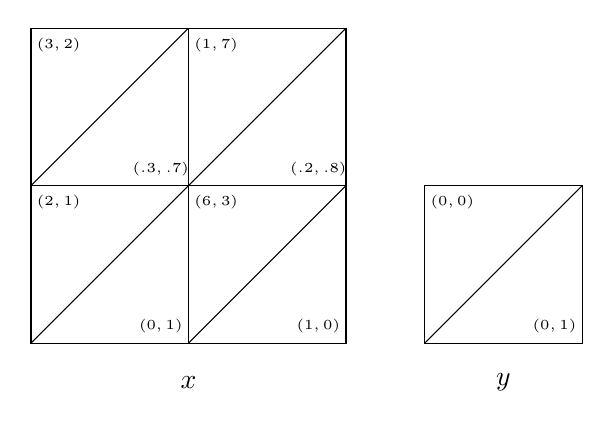
\begin{tikzpicture}
    \draw [rectangle] (0,0) -- (4,0) -- (4,4) -- (0,4) -- cycle;
    \draw (0,2) -- (4,2);
    \draw (2,0) -- (2,4);
    \draw (0,0) -- (4,4);
    \draw (0,2) -- (2,4);
    \draw (2,0) -- (4,2);
    \node (A) [right=10pt,below] at (0,4) {\tiny $(3,2)$};
    \node (B) [right=10pt,below] at (2,4) {\tiny $(1,7)$};
    \node [right=10pt,below] at (2,2) {\tiny $(6,3)$};
    \node [right=10pt,below] at (0,2) {\tiny $(2,1)$};
    \node [left=10pt,above] at (2,2) {\tiny $(.3,.7)$};
    \node [left=10pt,above] at (4,2) {\tiny $(.2,.8)$};
    \node (X) [left=10pt,above] at (2,0) {\tiny $(0,1)$};
    \node (Y) [left=10pt,above] at (4,0) {\tiny $(1,0)$};

    \draw [rectangle] (5,0) -- (7,0) -- (7,2) -- (5,2) -- cycle;
    \draw (5,0) -- (7,2);
    \node (C) [right=10pt,below] at (5,2) {\tiny $(0,0)$};
    \node (Z) [left=10pt,above] at (7,0) {\tiny $(0,1)$};


    \node at (2,-.5) {$x$};
    \node at (6,-.5) {$y$};
\end{tikzpicture}
\end{document}
